% This file was created with matplot2tikz v0.5.3.
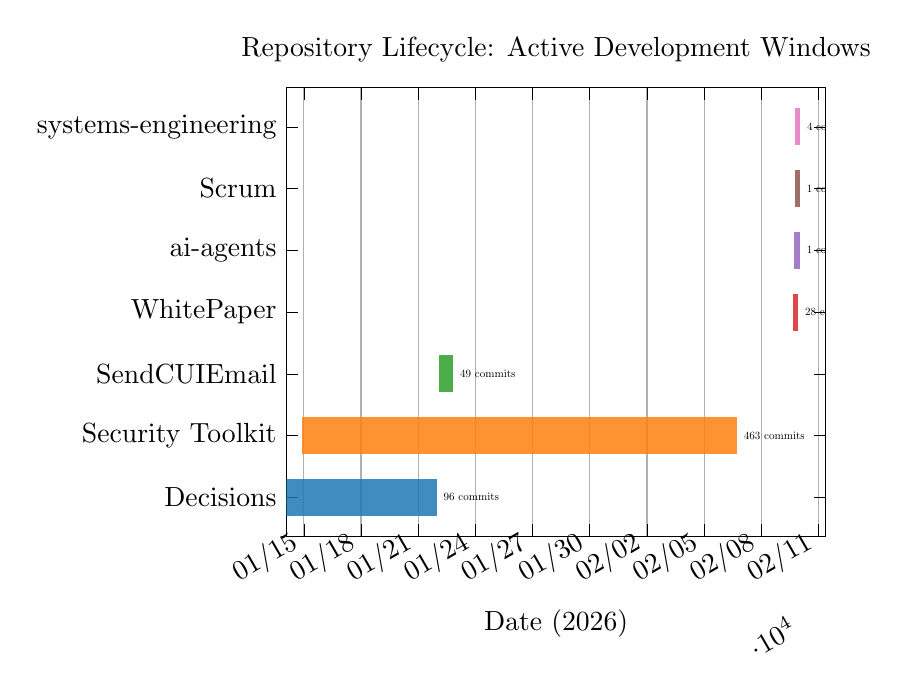
\begin{tikzpicture}

\definecolor{crimson2143940}{RGB}{214,39,40}
\definecolor{darkgray176}{RGB}{176,176,176}
\definecolor{darkorange25512714}{RGB}{255,127,14}
\definecolor{forestgreen4416044}{RGB}{44,160,44}
\definecolor{mediumpurple148103189}{RGB}{148,103,189}
\definecolor{orchid227119194}{RGB}{227,119,194}
\definecolor{sienna1408675}{RGB}{140,86,75}
\definecolor{steelblue31119180}{RGB}{31,119,180}

\begin{axis}[
tick pos=both,
title={Repository Lifecycle: Active Development Windows},
x grid style={darkgray176},
xlabel={Date (2026)},
xmajorgrids,
xmin=20467.0790625, xmax=20495.3893836806,
xtick style={color=black},
xtick={20468,20471,20474,20477,20480,20483,20486,20489,20492,20495},
xticklabel style={rotate=30.0,anchor=east},
xticklabels={01/15,01/18,01/21,01/24,01/27,01/30,02/02,02/05,02/08,02/11},
y grid style={darkgray176},
ymin=-0.63, ymax=6.63,
ytick style={color=black},
ytick={0,1,2,3,4,5,6},
yticklabels={
  Decisions,
  Security Toolkit,
  SendCUIEmail,
  WhitePaper,
  ai-agents,
  Scrum,
  systems-engineering
}
]
\draw[draw=none,fill=steelblue31119180,fill opacity=0.85] (axis cs:20467.0790625,-0.3) rectangle (axis cs:20474.9781018519,0.3);
\draw[draw=none,fill=darkorange25512714,fill opacity=0.85] (axis cs:20467.9158680556,0.7) rectangle (axis cs:20490.727662037,1.3);
\draw[draw=none,fill=forestgreen4416044,fill opacity=0.85] (axis cs:20475.0858796296,1.7) rectangle (axis cs:20475.8448148148,2.3);
\draw[draw=none,fill=crimson2143940,fill opacity=0.85] (axis cs:20493.6422916667,2.7) rectangle (axis cs:20493.9422916667,3.3);
\draw[draw=none,fill=mediumpurple148103189,fill opacity=0.85] (axis cs:20493.7296643519,3.7) rectangle (axis cs:20494.0296643519,4.3);
\draw[draw=none,fill=sienna1408675,fill opacity=0.85] (axis cs:20493.740474537,4.7) rectangle (axis cs:20494.040474537,5.3);
\draw[draw=none,fill=orchid227119194,fill opacity=0.85] (axis cs:20493.7412731481,5.7) rectangle (axis cs:20494.0412731481,6.3);
\draw (axis cs:20475.1281018519,0) node[
  scale=0.4,
  anchor=west,
  text=black,
  rotate=0.0
]{96 commits};
\draw (axis cs:20490.877662037,1) node[
  scale=0.4,
  anchor=west,
  text=black,
  rotate=0.0
]{463 commits};
\draw (axis cs:20475.9948148148,2) node[
  scale=0.4,
  anchor=west,
  text=black,
  rotate=0.0
]{49 commits};
\draw (axis cs:20494.0922916667,3) node[
  scale=0.4,
  anchor=west,
  text=black,
  rotate=0.0
]{28 commits};
\draw (axis cs:20494.1796643519,4) node[
  scale=0.4,
  anchor=west,
  text=black,
  rotate=0.0
]{1 commits};
\draw (axis cs:20494.190474537,5) node[
  scale=0.4,
  anchor=west,
  text=black,
  rotate=0.0
]{1 commits};
\draw (axis cs:20494.1912731481,6) node[
  scale=0.4,
  anchor=west,
  text=black,
  rotate=0.0
]{4 commits};
\end{axis}

\end{tikzpicture}
